\documentclass{article}
\usepackage[utf8]{inputenc}
\usepackage{amsmath, amsfonts, amsthm, amssymb, graphicx, geometry, lipsum}
\usepackage{hyperref}
\usepackage{indentfirst}
\usepackage[all,cmtip]{xy}
\usepackage{float}


\newtheorem{definition}{Definition}[section]
\newtheorem{lemma}{Lemma}[section]
\newtheorem{theorem}{Theorem}[section]
\newenvironment{theorem*}
 {\expandafter\def\expandafter\thetheorem\expandafter{\thetheorem*}\theorem}
 {\endtheorem}
\newtheorem{corollary}{Corollary}[theorem]
\newtheorem{proposition}{Proposition}[theorem]


\newcommand{\N}{\mathbb{N}}
\newcommand{\Z}{\mathbb{Z}}
\newcommand{\Q}{\mathbb{Q}}
\newcommand{\R}{\mathbb{R}}
\newcommand{\C}{\mathbb{C}}
\newcommand{\F}{\mathbb{F}}
\newcommand{\PP}{\mathbb{P}}
\newcommand{\HH}{\mathbb{H}}
\newcommand{\norm}[1]{\left\lVert #1 \right\rVert}
\newcommand{\innerp}[2]{\langle #1, #2 \rangle}

\DeclareMathOperator{\di}{d\!}




\title{Walking in a closed disk\\
{\Large University of Toronto}}
\author{Haocheng Sun}
\date{Fall 2024}

\begin{document}
\maketitle

Imagine all of you are selected to play a mathematical survival game. The settings are:
\begin{itemize}
    \item You are at the center of a closed disk whose radius is 20m.
    \item You receives a finite set of vectors $$M=\{\vec{v_1},\cdots,\vec{v_n}: \norm{\vec{v_i}}\leq 10, \sum_{i=1}^n\vec{v_i}=\vec{0}\}$$
    \item You can only walk by one vector in $M$ each time, you can only use one vector exactly once.
    \item If at any step you go outside the disk, you die. If you go back to the origin safely, you survive.
\end{itemize}

\begin{figure}[H]
    \centering
    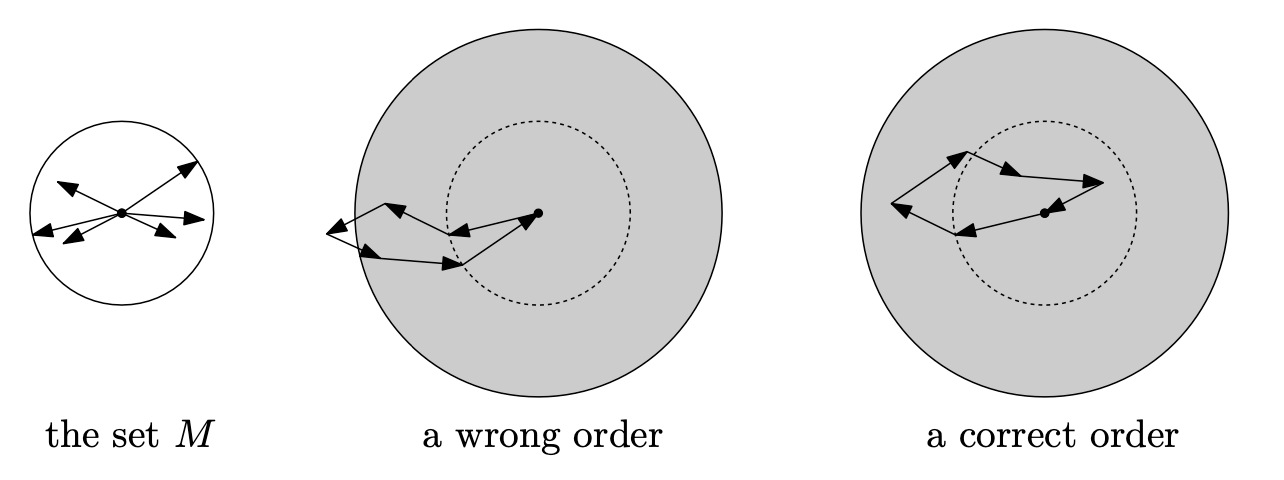
\includegraphics[scale=0.5]{images/Screenshot 2024-11-18 at 20.04.01}
    \caption{Example of the rules}
\end{figure}

Question: Is there a winning strategy?\\

Answer: Yes! For any $M$, we can always survive theoretically. The following theorem shows that a safe walk is possible for every
finite M, and it also works for yards that are d-dimensional balls.

\begin{theorem}
    Let $M$ be an arbitrary set of n vectors in $\R^d$ such that $\forall \vec{v}\in M. \norm{v}\leq 1$ and $\sum_{\vec{v}\in M}\vec{v}=\vec{0}$.
    Then it is possible to arrange all vectors of $M$ into a sequence $(v_1,v_2,\cdots,v_n)$ in such a way that $$\forall k\leq n. \norm{\vec{v_1}+\cdots+\vec{v_k}}\leq d$$
\end{theorem}

We start the proof with a simple general lemma.
\begin{lemma}
    Let $A\vec{x}=\vec{b}$ be a system of m linear equations in $n\geq m$ unknowns, 
    and let us suppose that it has a solution $\vec{x_0}\in[0,1]^n$. 
    Then there is a solution $\vec{x'}\in [0,1]^n$ in which at least $n-m$ components are 0's or 1's.
\end{lemma}

\begin{proof}
    We will prove this lemma by induction on $k=n-m$.
    \begin{itemize}
        \item Base case: $k=0$, in other words $n=m$.\\
        Just take $\vec{x'}=\vec{x_0}$, it automatically satisfies the requirement.
        \item Inductive step: Assume the lemma holds for $k-1$, then prove it holds for $k$.\\
        Then the solution space has dimension at least 1, so it contains a line passing through $\vec{x_0}$. 
        Since $\vec{x_0}\in [0,1]^n$, this line intersects the boundary of the cube $[0,1]^n$. Denote $\vec{y}$ as the intersection point. Thus $y_i\in\{0,1\}$ for some $i$. We now consider this $y_i$.\\
        Let us set up a new linear system with $n-1$ unknowns that is obtained from $A\vec{x}=\vec{b}$ by fixing the value $x_i=y_i$. 
        By deleting the component $y_i$ from the point $\vec{y}\in \partial[0,1]^n$, the new point satisfies the equation and ot is in $[0,1]^{n-1}$. 
        By induction hypothesis, there exists a point in $[0,1]^{n-1}$ with at least $n-m-1$ components equal to 0 or 1. By adding back the component $y_i$, we get a solution of the original system with at least $n-m$ components being 0 or 1
    \end{itemize}
\end{proof}

\begin{definition}
     Let $K=\{\vec{w_1},\cdots,\vec{w_k}\}$ in $\R^d$ with $k\geq d$ and $\norm{\vec{w_i}}\leq1$. We call such $K$ a \underline{good set} if there exist coefficients $alpha_1,\cdots,\alpha_k$ satisfying:
    \begin{itemize}
        \item $\alpha_i\in [0,1]$
        \item $\alpha_1\vec{w_1}+\cdots+\alpha_k\vec{w_k}=\vec{0}$
        \item $\alpha_1+\cdots+\alpha_k=k-d$
    \end{itemize}
\end{definition}

\begin{lemma}
    If $K$ is a good set of $k>d$ vectors, then there is some $i$ such that $K\setminus\{\vec{w_i}\}$ is a good set of $k-1$ vectors.
\end{lemma}
\begin{proof}
We consider the following system of linear equations for unknowns \(x_1, \ldots, x_k\):
\begin{align}
    x_1 w_1 + x_2 w_2 + \cdots + x_k w_k &= 0 \tag{*} \\
    x_1 + x_2 + \cdots + x_k &= k - d - 1. \tag{**}
\end{align}
Here (*) is an equality of two \(d\)-dimensional vectors and thus it actually represents \(d\) equations. The last equation (**) is like the third condition of the definition, except that the right-hand side is \(k - d - 1\); this is a preparation for showing that a suitable subset of \(k - 1\) vectors in \(K\) is good.

The above system has \(d + 1\) equations for \(k\) unknowns. If \(\alpha_1, \ldots, \alpha_k\) are the coefficients witnessing that \(K\) is good, then by setting \(x_i := \frac{k - d - 1}{k - d} \alpha_i\), we obtain a solution of (*), (**) lying in \([0, 1]^k\).

Thus by the lemma there is also a solution \(\tilde{x} \in [0, 1]^k\) with at least \(k - d - 1\) components equal to \(0\) or \(1\). We want to see that at least one component of \(\tilde{x}\) has to be \(0\). Indeed, if all the \(k - d - 1\) components guaranteed by the lemma happen to be \(1\), then all of the remaining \(d + 1\) components must be \(0\), since all components add up to \(k - d - 1\) by (**).

Now it is easy to check that for any index \(i\) with \(\tilde{x}_i = 0\) the set \(K \setminus \{w_i\}\) is good. Indeed, the remaining components of \(\tilde{x}\) can be used in the role of the \(\alpha_i\) in the definition of a good set. This proves the lemma.
\end{proof}

\begin{lemma}
    Follow the setting of $K$ above, $\norm{\vec{w_1}+\cdots+\vec{w_k}}\leq d$
\end{lemma}
\begin{proof}
    \begin{align*}
        \norm{\sum_{i=1}^k\vec{w_i}} &= \norm{\sum_{i=1}^k\vec{w_i}-\sum_{i=1}^k\alpha_i\vec{w_i}}\\
        &= \norm{\sum_{i=1}^k(1-\alpha_i)\vec{w_i}}\\
        &\leq \sum_{i=1}^k(1-\alpha_i)\norm{\vec{w_i}}\\
        &\leq \sum_{i=1}^k(1-\alpha_i)\\
        &= d
    \end{align*}
\end{proof}


\begin{proof}[Proof of the theorem]
    We will use induction on $n$.
    \begin{itemize}
        \item Base case: $n=2$.\\ 
        This is trivial. Just notice that $n$ cannot be one because we cannot go back to origin. And for $n=2$, we can only have $\vec{v_1}=-\vec{v_2}$.
        \item Inductive step: Assume theorem holds for $n-1$, we prove it holds for $n$.\\
        We start with the set $M_n=M$, which is obviously a good set. By the second lemma, we can find a vector in $M$ denoted as $\vec{v_n}$. Such that $M_{n-1}=M_n\setminus\{\vec{v_n}\}$ is a good set. 
        Similarly, having constructed the good set $M_k$, we find can find a vector $\vec{v_k}\in M_k$ such that $M_{k-1}=M_k\setminus\{\vec{v_k}\}$ is a good set. By the third lemma, done.
    \end{itemize}
\end{proof}


\begin{theorem*}
    In the plane, for any such set $M$, there is a way to arrange the path lies in the radius $\frac{\sqrt{5}}{2}$, this is the smallest possible radius.
\end{theorem*}

\textbf{Open Question}: What is the smallest possible radius for the case of general d-dimension sphere?




\end{document}